Het \index{Hi\"erarchisch Netwerk Ontwerp}\index{HND}Hi\"erarchisch Netwerk Ontwerp is een oorspronkelijk door Cisco bedacht model. Dit netwerk model bestaat uit 3 lagen en wordt daarom ook wel het Three-Tier-model genoemd. De access laag, de distributie laag en de core laag zoals weergegeven in figuur \ref{HND}.

\begin{figure}[H]
\centering
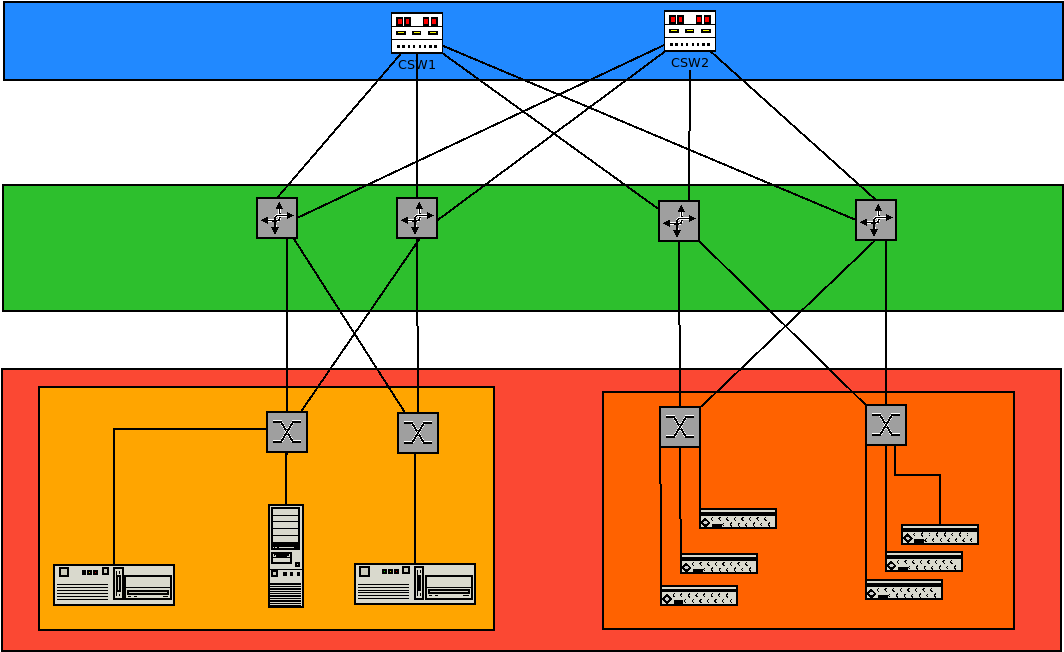
\includegraphics[width=\linewidth]{HND.png}
\caption{Blauw is de core, groen is de distributie laag en rood is de access laag met links de gebruikers en rechts der servers}
\label{HND}
\end{figure}

Op de access laag (rood in bovenstaande tekening) worden over het algemeen access switches gebruikt (OSI-layer 2), maar ook routers kunnen op deze laag voorkomen (bijvoorbeeld de Top-of-Rack switches). Dit zijn "goedkope" switches die zorgen dat er voldoende poorten zijn voor alle gebruikers en alle servers in het netwerk. VLANs worden vaak op de access laag gebruikt om broadcast domains van elkaar te scheiden. De kosten per port is hier vaak de belangrijkste afweging. Het uitvallen van een access switch treft alleen de aangesloten gebruikers en heeft verder geen invloed op de rest van de organisatie. Dit is niet het geval als het een access switch in de serverruimte is waar meerdere servers aan hangen.

Op de distributie laag (groen in bovenstaande tekening) vinden we de meer intelligente devices die bijvoorbeeld afdelingen binnen een organisatie van elkaar scheiden door bijvoorbeeld firewalling, IP-routing en filtering. Ook QoS wordt op vaak op deze laag geregeld. Verbindingen naar andere kantoren van een organisatie behoren ook tot de distributie laag. 

De core laag (blauw in bovenstaande tekening) bevat vaak de duurste netwerk onderdelen omdat deze moeten zorgen dat er grote hoeveelheiden data op een snelle manier verdeeld worden over de verschillende distributie componenten. Vaak zijn de core componenten redundant uitgevoerd. De hoogste netwerksnelheden per port vinden we vaak in deze laag. Omdat snelheid hier de fundamentele factor is vind hier geen of nauwelijks filtering plaats. Op deze laag kunnen we switches of routes (Layer 2 of 3 technologie) tegen komen.

Dit model om een datacenter op te zetten is vooral bedoeld als er veel north-south verkeer is. Dat wil zeggen dataverkeer dat van boven naar beneden door het model gaat, er is dan dus veel verkeer van binnen naar buiten en omgekeerd. Denk hierbij aan een datacenter dat veel faciliteiten aanbiedt aan gebruikers die niet zelf in het datacenter zitten zoals bijvoorveel webservers.

Elke core switches is verbonden met elke distributie-switch en elke distributie-switch is redundant verbonden met de access-switches. Door deze redundantie kan er data in rondgangen (loops) door het netwerkgaan. Om dit tegen te gaan is er het spanning-tree protocol (IEEE802.1d,w,s en IEEE802.1q). Het juist congfigureren van het spanning-tree protocol is dan ook een must in een Three-tier netwerk.
